\begin{frame}{Experiment 4}
\setbeamercovered{invisible}
\fontsize{11pt}{15}\selectfont
\vspace{-0.5cm}
\only<2-4>{\large\textbf{Results:\\}}
\only<1>{{\large Expected the participants to \textbf{perform better} with the tool after \textbf{training with object relatives} rather than with subject relatives.}}
\pause
\only<2>{
\vspace{-0.6cm}
\begin{columns}
    \begin{column}{0.5\textwidth}
    \vspace{-0.3cm}
    \begin{figure}
    \centering
    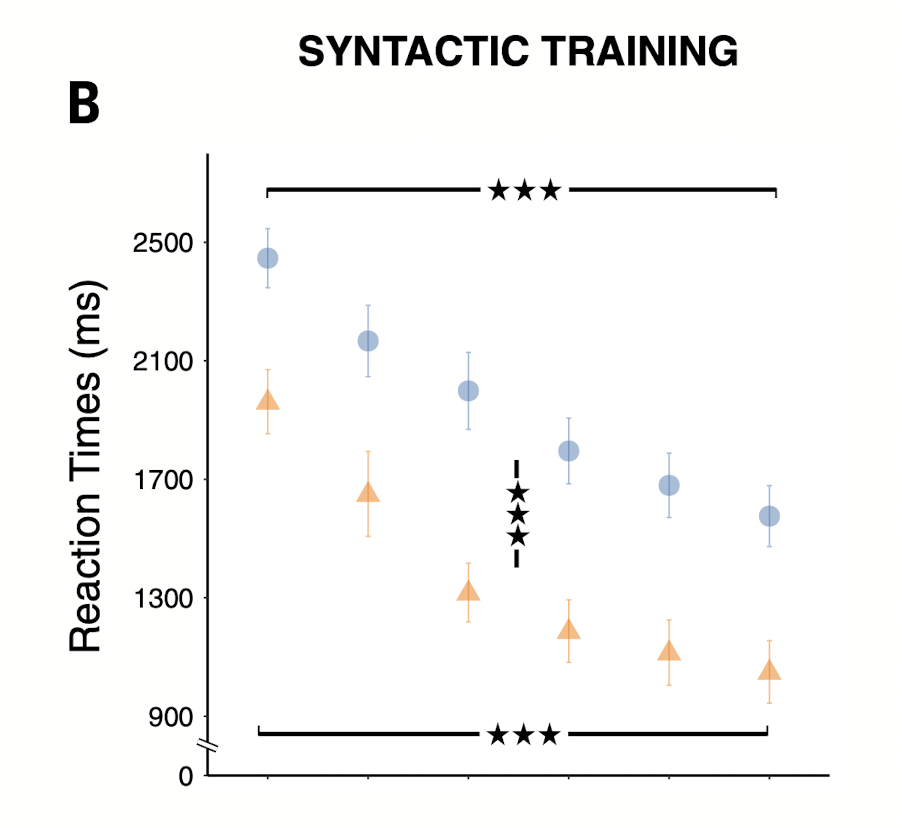
\includegraphics[width=5.6cm]{images/paper_pics/fig4B.png}
    %\caption*{}
    \label{fig:label11}
\end{figure}
    \end{column}
    \begin{column}{0.5\textwidth}
    \vspace{0.7cm}
        \begin{figure}
    \centering
    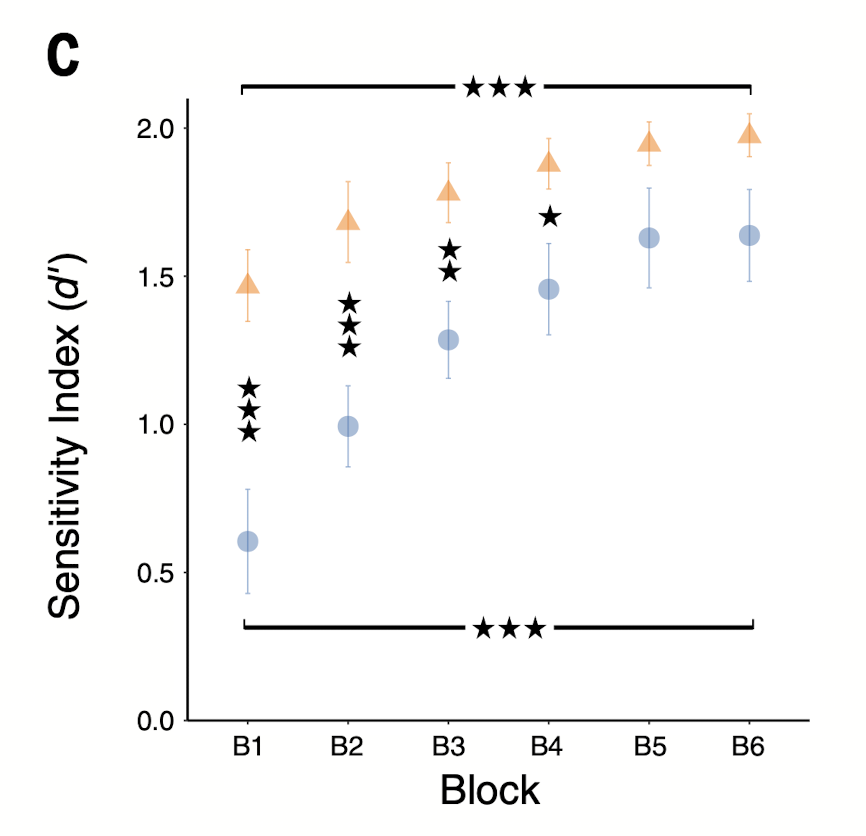
\includegraphics[width=5.6cm]{images/paper_pics/fig4C.png}
    %\caption*{}
    \label{fig:label12}
\end{figure}
    \end{column}
\end{columns}
\vspace{-0.7cm}
\hspace{1cm}{\footnotesize Both groups improved in processing relative sentences during training.}
}
\pause
\only<3>{
\begin{figure}
    \centering
    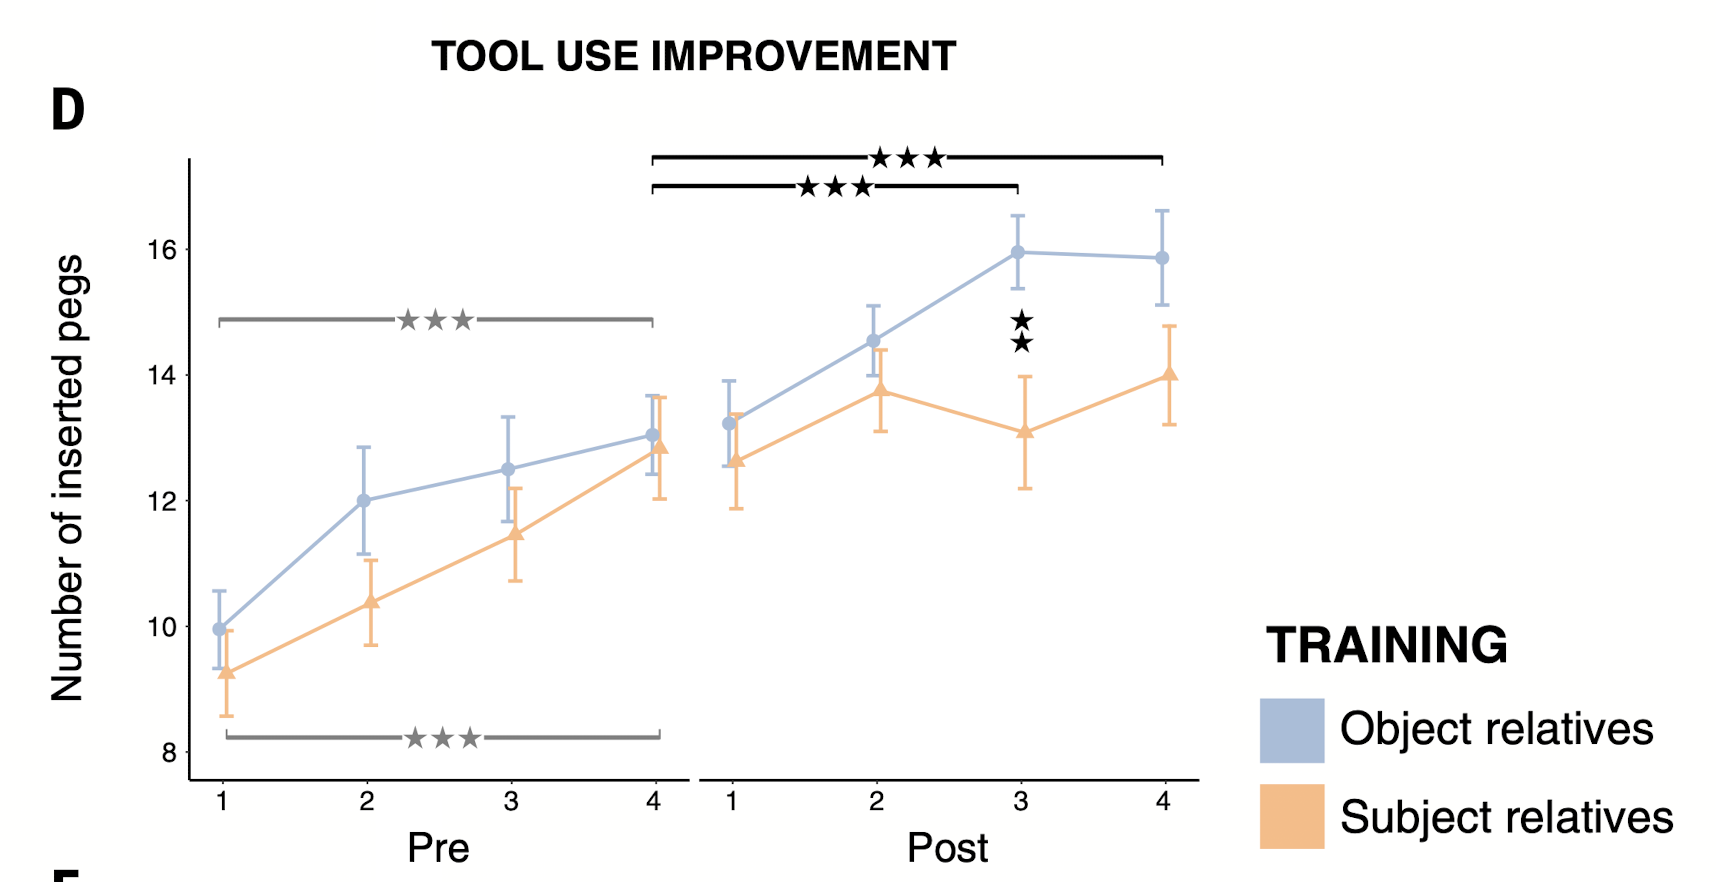
\includegraphics[width=10cm]{images/paper_pics/fig4D.png}
    \vspace{0.2cm}
    \caption*{{\footnotesize Participants who trained with \textbf{object relatives} kept improving significantly with the tool.}}
    \label{fig:label12}
    \end{figure}
    }

\only<4>{
\begin{itemize}
\vspace{0.2cm}
    \item Training with subject relatives did not change participants’ motor performance.
\end{itemize}
    
}


\end{frame}